\paragraph{Description}
Refer back to experimental design
\paragraph{Conclusion}
Expect to be linear, see that it's linear. 

\begin{figure}[h]\centering
    \begin{subfigure}{0.45\textwidth}
        \begin{tikzpicture}
            \begin{axis}[
                % width = 14cm, height = 6cm,
                ymin = 0,xmin=0,
                xlabel = {Offset [mm]}, ylabel = {Maximum displacement [nm]}
            ]
                \addplot+[ only marks] table [ col sep=comma, y expr = 1e9*\thisrowno{1}]
                    {Modelling/Forces/Offsets/spigot_maxima.csv};
                \addlegendentry{Spigot}
                \addplot+[ only marks] table [ col sep=comma, y expr = 1e9*\thisrowno{1}]
                    {Modelling/Forces/Offsets/stem_maxima.csv};
                \addlegendentry{Stem}
                \addplot+[ only marks] table [ col sep=comma, y expr = 1e9*\thisrowno{1}]
                {Modelling/Forces/Offsets/collar_maxima.csv};
            \addlegendentry{Collar}
            \end{axis}
        \end{tikzpicture}
        \caption{Maximum displacement.}
    \end{subfigure}\hfill
    \begin{subfigure}{0.45\textwidth}
        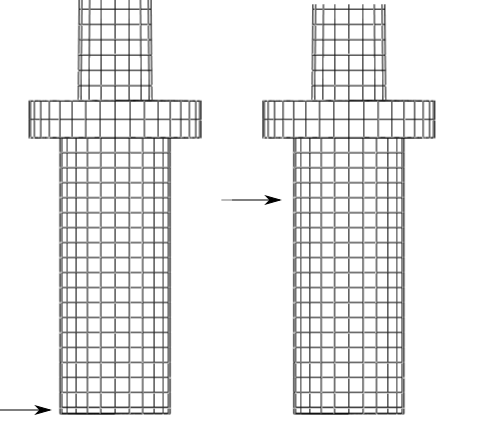
\includegraphics[width=1\textwidth]{figures/load-position.png}
        \caption{Offset from the base of the spigot. Starting at about 1mm on the left.}
    \end{subfigure}
    \caption{ (a) shows maximum displacement for the same stimulus applied at increasing offset from base of spigot. (b) is a visual aid to understand of what is meant by increasing the offset from the base of the spigot.}
    \label{fig:offset-from-base}
\end{figure}